\documentclass[11pt]{article}
\usepackage[spanish]{babel}
\usepackage{graphicx}
\graphicspath{ {./imagenes/} }

\title{Proyecto \#2: Programación paralela\\
Algoritmo de Dijkstra\\
\large Estructura de datos y algoritmos II}

\author{Cabello, Sofía
\and López, Ricardo
\and Núñez, Diego}

\begin{document}

\maketitle{}

\section{Algoritmo utilizado y su implementación }


Primero que nada, es importante aclarar que nos basamos en código encontrado en \cite{Matloff2012} al que se le hicieron algunas modificaciones, ya que se generaba una condición de carrera que será explicada más adelante.
\par 
¿Cómo correr el programa? El programa recibe dos parámetros desde la terminal, uno para indicar el número de nodos que tendrá el grafo aleatorio (llamado nv dentro del programa) y otro para indicar si se deben imprimir los resultados. Aunque esta última opción parece un poco extra o tonta, fue muy útil para las pruebas de rendimiento.
\par 
El programa comienza llenando la matriz de adyacencia del grafo. Como el programa crea grafos ponderados bidireccionales, no se ingresan valores negativos a la matriz. Primero se llena una mitad y después los valores son copiados a la otra, ya que la matriz debe ser simétrica.
\par 
Después, se inicializan los valores de un arreglo de nv espacios que indica si un nodo todavía no ha sido visitado. Al nodo 0 le corresponde el espacio 0 de este arreglo, al 1 el espacio 1 y así sucesivamente hasta nv-1. Cuando existe un valor de 1, entonces el nodo todavía no ha sido visitado. A este arreglo se le conoce como no notDone.
\par
Junto al arreglo anterior se inicializan los valores de otro arreglo llamado mind, que almacena las distancias mínimas almacenadas hasta el momento hacia cada nodo. Por defecto, estas distancias se inicializan con el valor de la arista que conecta directamente a cualquier nodo con el nodo 0. Además, este arreglo almacena datos de tipo usigned, ya que esta versión del algoritmo que no utiliza una cola de prioridad no funciona con pesos negativos. 
\par
Teniendo todo listo comienza el algoritmo en sí. Se encuentra el constructor parallel, lo que significa que a partir de este punto se utilizarán varios hilos. Primero, se inicializan tres variables, step, mymv y mymd. La primera variable indica que nodo se está revisando en un momento. Cada nodo es revisado una vez, por esta razón step va desde 0 hasta nv-1. La segunda y la tercera sirven para almacenar de manera local para los hilos cual es el nodo más cercano al nodo inicial que han encontrado de manera individual. 
\par
Después, en un bloque single, se inicializa los valores de mv y md. Estas variables almacenan el nodo más cercano al nodo inicial de entre todos los encontrados por todos los hilos. La variable md se inicializa en -1 (Que, como las distancias son de tipo unsigned, en realidad representa el mayor entero posible) y mv en 0. Esto es así ya que la distancia mínima encontrar al inicio del algoritmo es presuntamente infinita y el vértice hacia el que hay esa distancia es presuntamente inexistente hasta que se indique lo contrario.
\par
Después, en una estructura omp for, cada hilo trabaja con un subconjunto de los nodos adyacentes al nodo 0, cada uno determina cual es el más cercano de su subconjunto. Luego, en una estructura critical, cada hilo pasa uno por uno a revisar si su menor valor encontrado es menor al ya existente. Si es así, se actualizan mv y md para referir al nodo más cercano en la iteración.
\par
En una estructura single, se marca a este nuevo nodo más cercano como revisado, así que en la siguiente iteración ya no podrá ser seleccionado como el nodo más cercano al inicial.
\par
Finalmente, en un ciclo for también paralelizado, se calculan distancias hacia todos los demás nodos y si es menor a la distancia más corta ya existente, se actualiza. 
\par
En este punto es donde se generaba la condición de carrera. OpenMP no asegura la manera ni el orden en cómo se ejecutarán las iteraciones de una estructura for. Por esta razón, un hilo podía terminar su parte primero y llegar a esta sección antes de que el otro, actualizando las distancias antes de que los demás hilos propusieran un nodo para ser el más pequeño en general. Para arreglar esto, se agregó una barrera después del critical, de esta manera se espera que todos los hilos actualicen mv y md si lo requieren antes de continuar. 
\par
En la siguiente iteración se repite el proceso, solo que esta vez ya estará marcado el nodo más cercano que se utilizó en la iteración anterior, por lo que ahora se ocupará el segundo más cercano y así sucesivamente hasta que no haya más nodos adyacentes al nodo inicial.


\begin{figure}[!htbp]
\centering
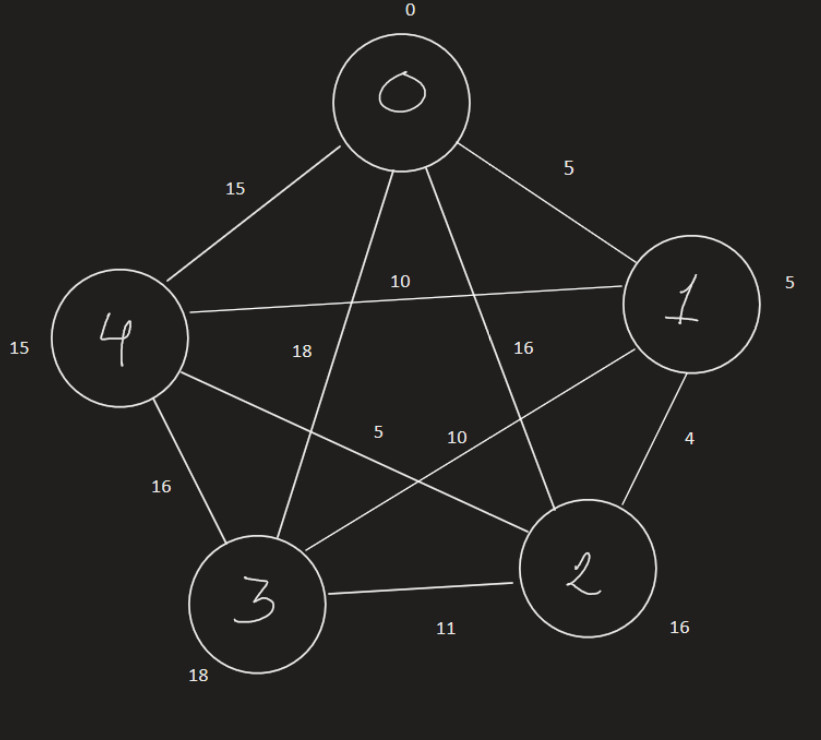
\includegraphics[scale = .5]{grafos1}
\caption{Grafo inicial}
\end{figure}

\begin{figure}[!htbp]
\centering
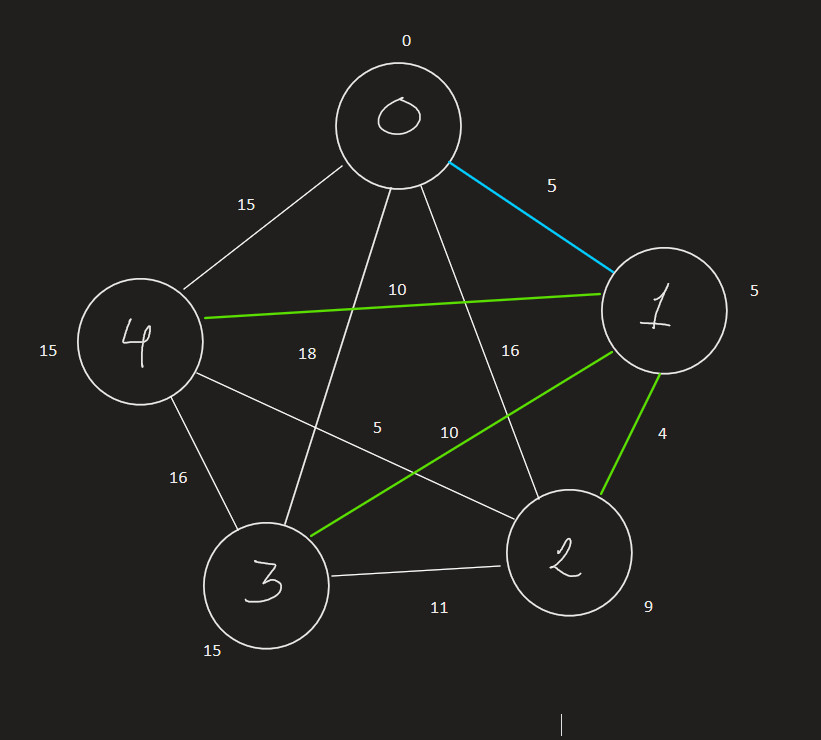
\includegraphics[scale = .5]{grafos2}
\caption{Primero se visita al nodo al nodo adyacente más cercano al origen.}
\end{figure}


\begin{figure}[!htbp]
\centering
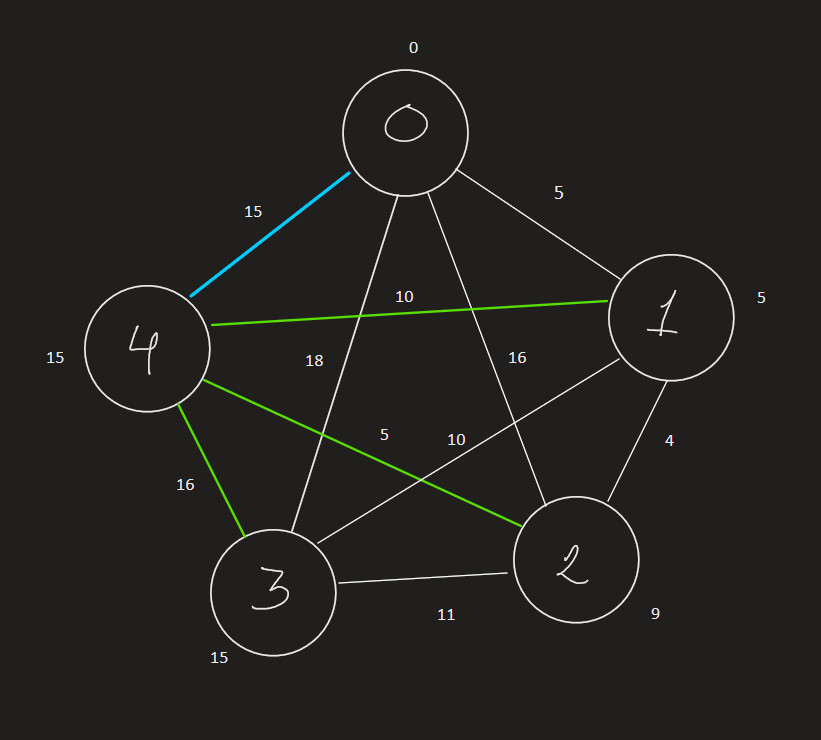
\includegraphics[scale = .5]{grafos3}
\caption{Después se visita el segundo más cerca.}
\end{figure}

\begin{figure}[!htbp]
\centering
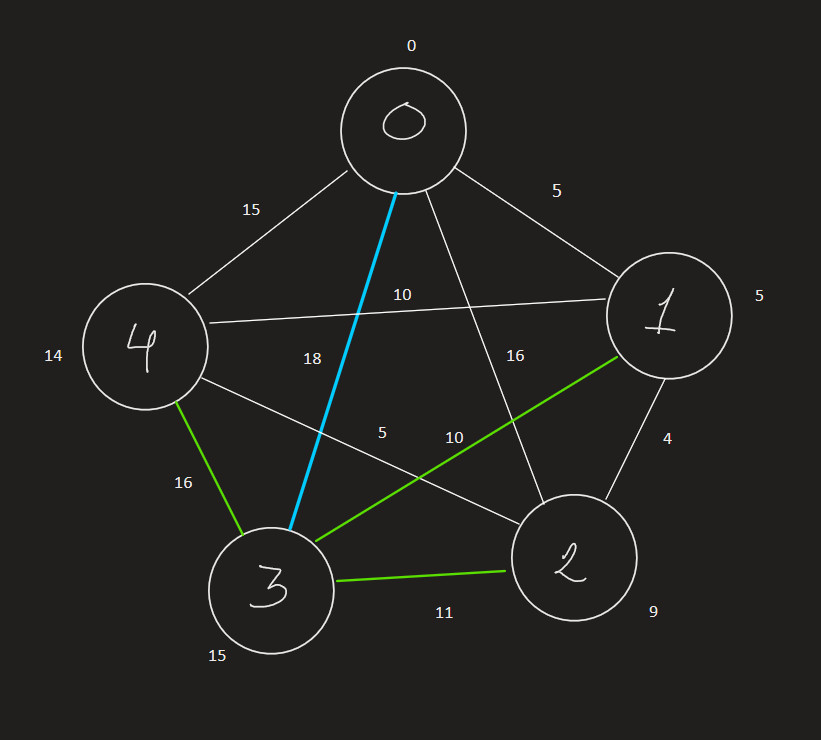
\includegraphics[scale = .5]{grafos5}
\caption{El algoritmo finaliza una vez que se visitó el más lejano.}
\end{figure}

\section{Paralelización del Algoritmo}
\subsection{Nivel de paralelismo}
Muchos algoritmos realizan cálculos atravesando iterativamente una gran estructura de datos por medio de un bucle. Por lo general, un bucle se ejecuta secuencialmente, lo que significa que los cálculos de la i-ésima iteración no se inician antes de que se completen todos los cálculos de la (i - 1) ésima iteración. Este esquema de ejecución se denomina ciclo secuencial.
\par
Si no hay dependencias entre las iteraciones de un bucle, las iteraciones se pueden ejecutar en un orden arbitrario y también se pueden ejecutar en paralelo por diferentes procesadores. Entonces, dicho bucle se denomina bucle paralelo.
\par 
En el caso del programa del Algoritmo de Dijkstra, cada hilo ejecuta una o más de las iteraciones, es decir, asume la responsabilidad de uno o más valores de i. Es por esto que podemos afirmar que el nivel de paralelismo que se maneja es a nivel de ciclo.

\subsection{Métricas de desempeño}
El principal propósito de escribir programas paralelos es aumentar el rendimiento con respecto a su contraparte secuencial. Para poder medir esto se establecieron las métricas de desempeño, que proporcionan elementos para decidir si los programas valen la pena o no.
\par
El tiempo de procesamiento del programa del Algoritmo de Dijkstra fue tomado en tres distintos procesadores con el mismo grafo para todos los casos. Los procesadores utilizados fueron los siguientes:
\par
Procesador 1: Intel i5, 2.50 GHz, 4 núcleos
\par
Procesador 2: Intel i5, 1.4 GHz, 4 núcleos
\par
Procesador 3: Intel i7, 2 GHz, 8 núcleos
\par
Los resultados obtenidos se muestran a continuación:

\begin{figure}[!htbp]
\centering
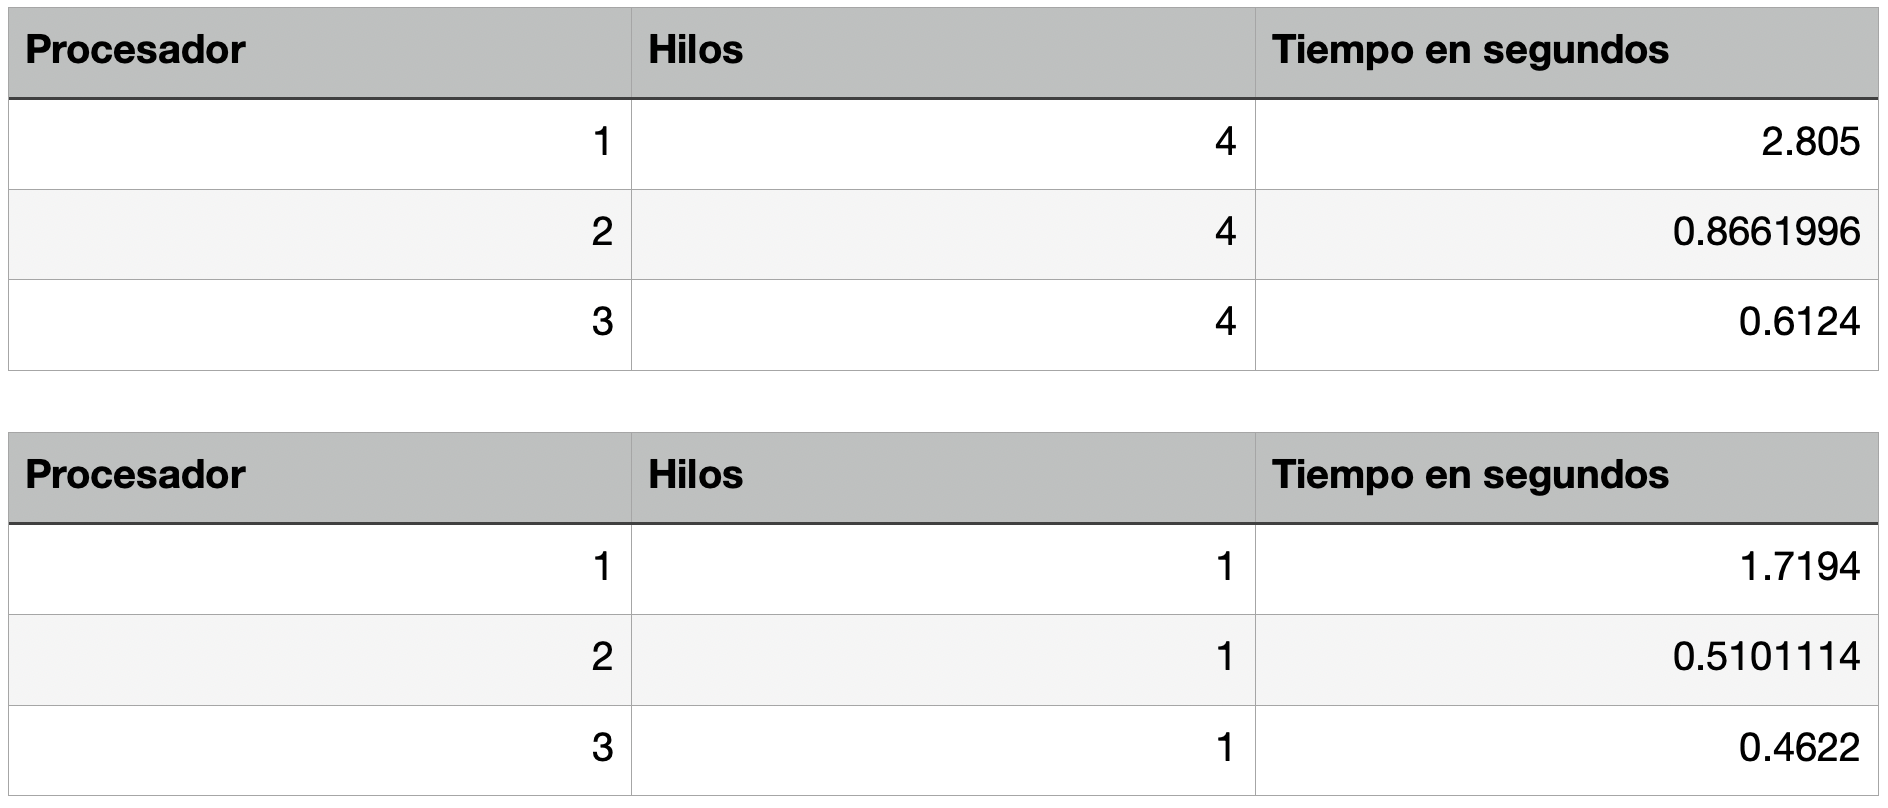
\includegraphics[scale = .5]{tiempo}
\caption{Para la toma del tiempo se utilizó la función omp\_get\_wtime() de la biblioteca omp.h}
\end{figure}

\subsubsection{Speedup}
Para el análisis de programas paralelos, una comparación con el tiempo de ejecución de una implementación secuencial es especialmente importante para ver el beneficio del paralelismo.
\par
El speedup de una implementación paralela expresa el ahorro de tiempo de ejecución que se puede obtener utilizando una ejecución paralela en n procesadores en comparación con la mejor implementación secuencial.
\par
Para el programa del Algoritmo de Dijkstra se obtuvo lo siguiente:

\begin{figure}[!htbp]
\centering
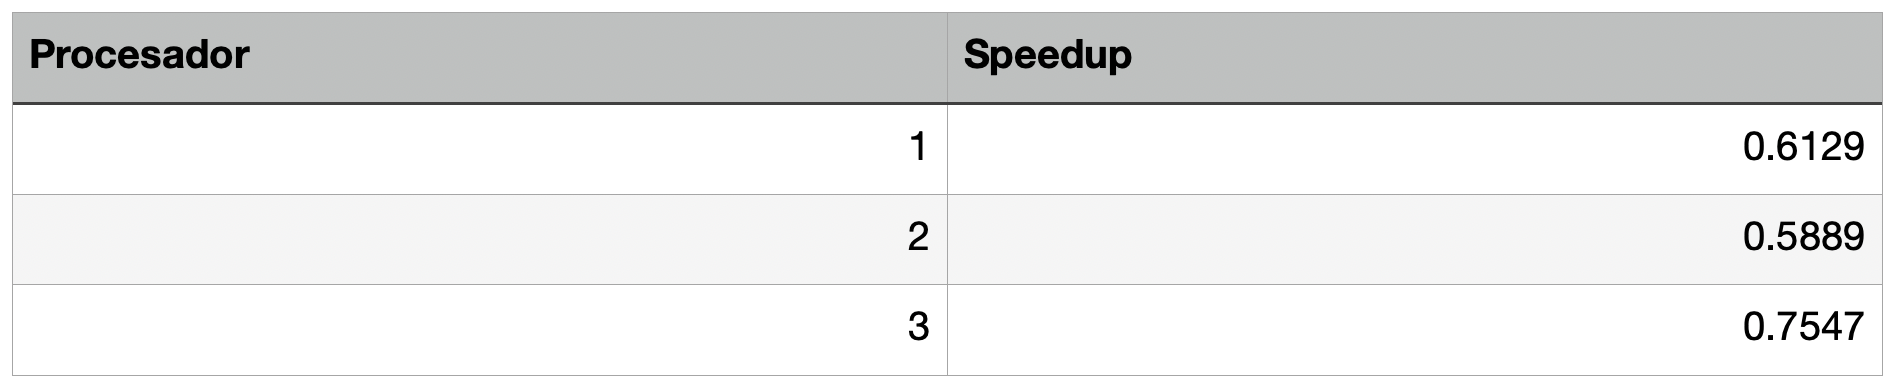
\includegraphics[scale = .5]{speedup}
\end{figure}

En los tres procesadores se observa que el valor del speedup es menor que la unidad. Esto quiere decir que el algoritmo ejecutado en forma paralela no presenta una mejora en cuanto al tiempo de ejecución, al contrario, hace que el programa se ejecute más lento.

\subsubsection{Eficiencia}
La eficiencia se define como la medida de la fracción de tiempo en la que cada procesador es usado para resolver el problema en cuestión de forma útil. En otras palabras, refleja el aprovechamiento de los recursos de hardware del sistema.
\par
Los cálculos de eficiencias obtenidos fueron los siguientes:

\begin{figure}[!htbp]
\centering
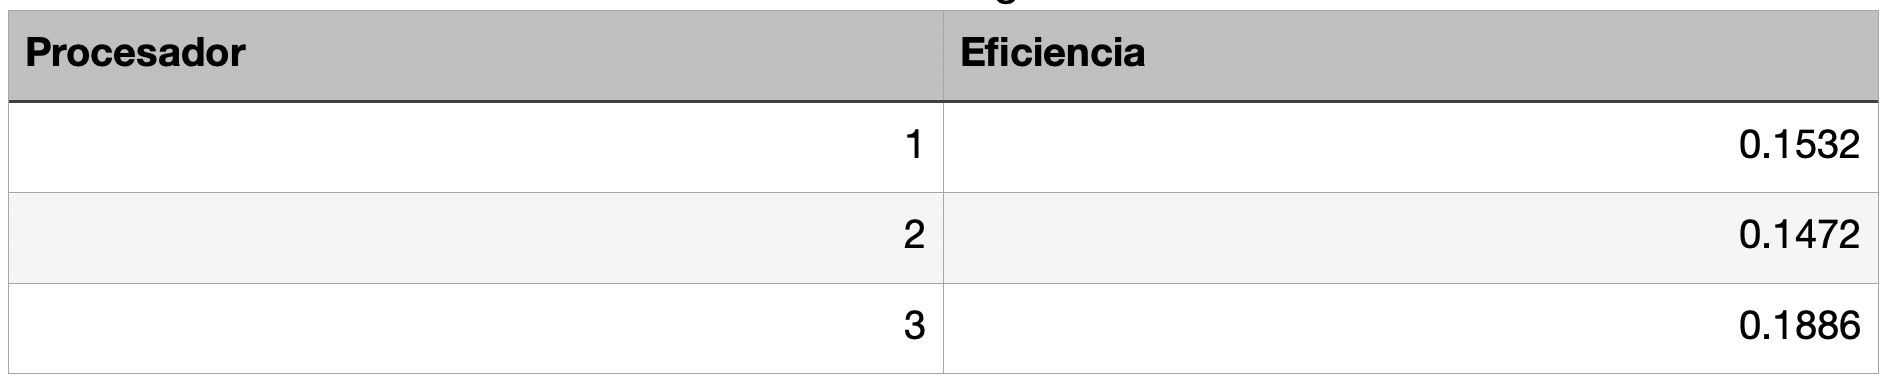
\includegraphics[scale = .5]{eficiencia}
\end{figure}

Si nuestros procesadores se utilizan de forma eficiente se espera que el tiempo de ejecución dedicado por cada procesador por el número de procesadores sea igual al tiempo de ejecución en un sólo procesador. Esto quiere decir que se requiere un valor cercano a la unidad. En base a los resultados obtenidos, se puede observar que están más cercanos a 0 que a 1, por lo que el programa no tiene una buena eficiencia.

\subsubsection{Fracción serial}
La fracción serial relaciona el speedup y la eficiencia con el propósito de tomar en cuenta otros factores además del tiempo.
\par
Los resultados se muestran a continuación:

\begin{figure}[!htbp]
\centering
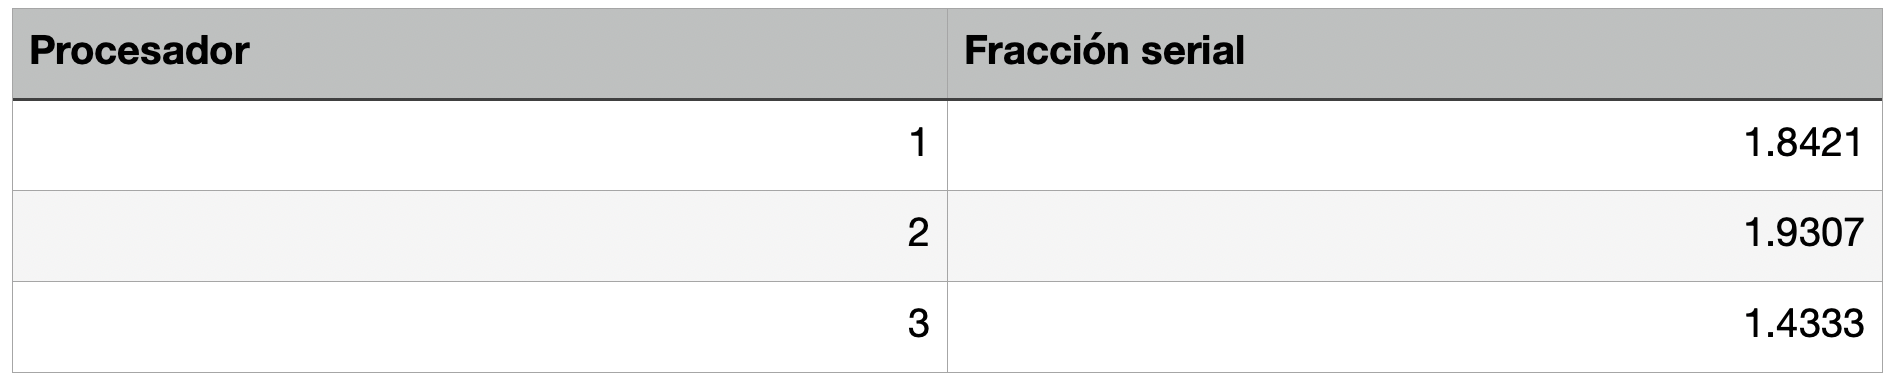
\includegraphics[scale = .5]{fraccion}
\end{figure}

Después de obtener las métricas de desempeño podemos afirmar que el programa no presenta una mejora en cuanto a su versión secuencial. En un apartado posterior se hará un análisis más profundo de esto.

\subsection{Formas de comunicación}
Una región paralela es ejecutada por varios hilos que acceden a los mismos datos compartidos, por lo que es necesaria la sincronización para proteger las regiones críticas o evitar la condición de carrera. OpenMP ofrece varios constructores que se pueden utilizar para la sincronización y coordinación de hilos dentro de una región paralela. El constructor critical especifica una región crítica que solo puede ser ejecutada por un único hilo a la vez. 
\par
Dentro del código del Algoritmo de Dijkstra encontramos distintas partes en donde se presentan regiones críticas, es por ello que se utiliza el constructor critical y otros constructores que ayudan a la sincronización de hilos como single y barrier.

\subsection{Granularidad}
El tiempo de cálculo de una tarea se denomina granularidad: las tareas con muchos cálculos tienen una granularidad de grano grueso, las tareas con solo unos pocos cálculos son de grano fino. 
\par
En el caso del programa del Algoritmo de Dijkstra se presenta una granularidad de tipo fina, ya que en cada región paralela hay pocas instrucciones. Lamentablemente, esto afecta directamente al desempeño del programa debido a que hay una gran sobrecarga de comunicación y sincronización de los hilos.

\section{Pruebas}

\par
Se realizaron múltiples pruebas para analizar el rendimiento del programa. Para ellos fue necesario ejecutar en tres diferentes procesadores las diferentes versiones y analizar su comportamiento. 

\par
Empezaremos comparando a la versión paralela consigo misma. n la Figura 2 se puede ver que sin importar el procesador que se use, la tendencia es que al usar más hilos, aumenta el tiempo de ejecución del programa. Esto se hace más evidente dependiendo del número de núcleos con los que cuente la computadora.  

\begin{figure}[!h]
\centering
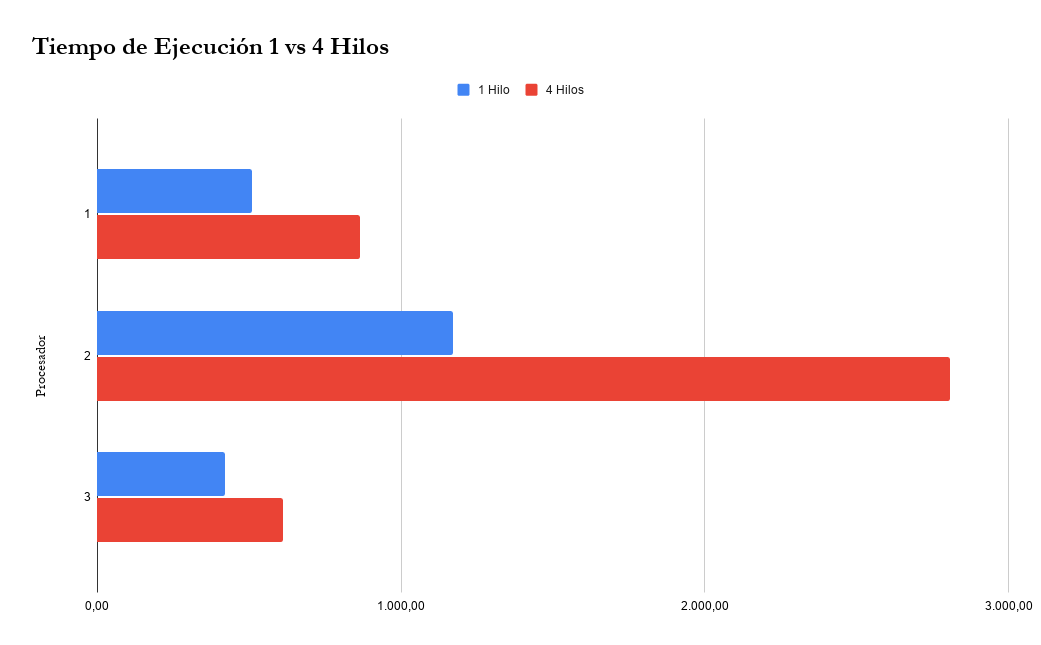
\includegraphics[width=0.9\linewidth]{hil1v4.png}
  \caption{Ejecución en segundos usando 3 diferentes procesadores.}
\end{figure}

\paragraph{}
Ahora, si comparamos el rendimiento de la versión serial contra la paralela (usando 4 hilos, es claro que el algoritmo linear es más eficiente. La diferencia crece conforme aumenta el tamaño de los datos. 

\begin{figure}[!h]
\centering
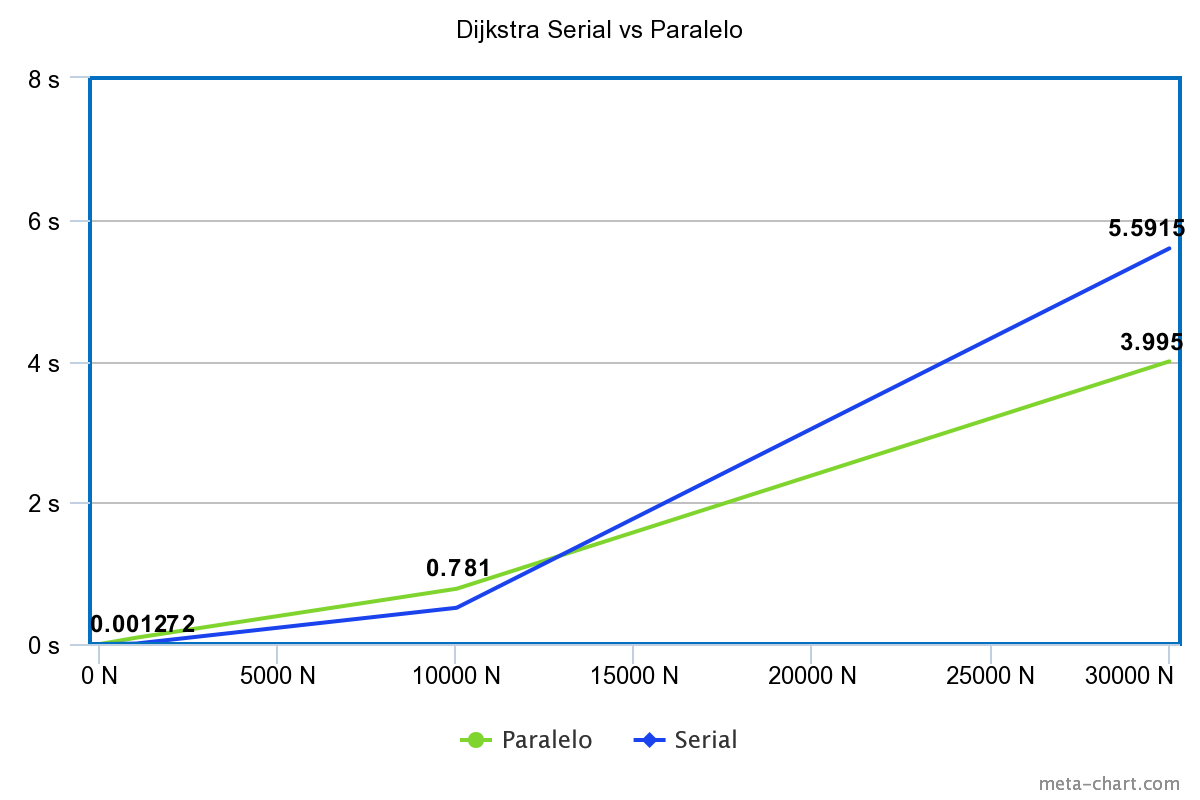
\includegraphics[width=0.9\linewidth]{tablas.png}
  \caption{Rendimiento de programa serial vs paralelo.}
\end{figure}

\begin{figure}
\centering
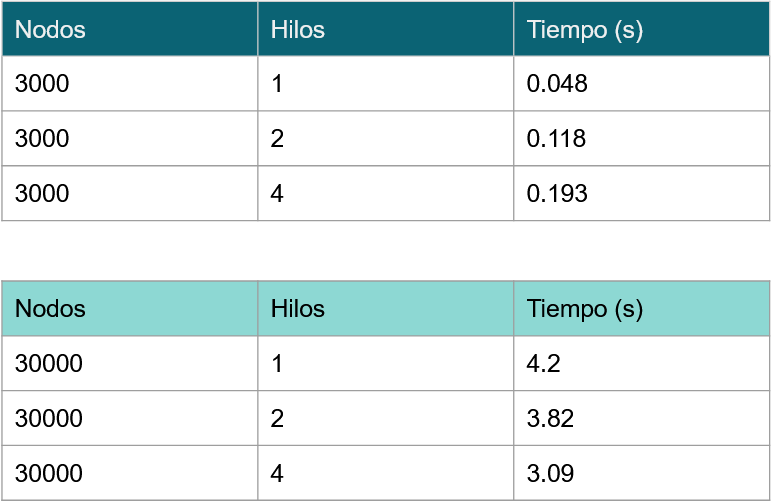
\includegraphics[width=0.9\linewidth]{tablas1.png}
  \caption{Rendimiento de programa paralelo con diferente cantidad de nodos.}
\end{figure}


\paragraph{}
Algo importante a notar aquí es que el tiempo de ejecución depende del tamaño del problema, es decir, cuando tenemos pocos nodos resulta poco conveniente implementar paralelismo. Mientras más crece la camtidad de nodos con la que se va a trabajar, la versión paralela del algoritmo se vuelve más eficiente, como lo indican las tablas de la Figura 9. 
\par 
Hay diferentes factores que pudieran estar favoreciendo este comportamiento. El primero de ellos es la sección crítica presente en el código. Es neesaria por que en cada iteración, los hilos calculan sus valores de distancia mínima local a un cierto vértice, y luego actualizan los valores globales. Dado que la actualización debe ser atómica (sólo puede ser realizada por un hilo), esto provoca cierta serialización del programa.
\par
Otro factor podría que es posible que ocurra False Sharing durante la ejecución. Esto se refiere a que cuando una parte del programa intenta acceder en el ciclo a datos que no serán alterados pero que comparten bloques de caché con datos que sí lo son, como en este caso las variables de distancia,el protocolo de caché puede forzar al programa a recargar todo el bloque a pesar de no ser extrictamente necesario, lo cual ocasiona esperas en la memoria además de perder eficiencia de procesador.

\par
Por último, se puede considerar el balance de carga, particularmente en el ciclo. En realidad no se está definiendo una partición específica de las iteraciones que le corresponden a cada hilo del programa. Por un lado, las particiones grandes son buenas, debido a que hay menos sobrecarga: cada vez que un hilo termina un fragmento, debe pasar por la sección crítica,que serializa nuestro programa paralelo y, por lo tanto, ralentiza las cosas. Por otro lado, si los tamaños de las particiones son grandes, entonces hacia el final del trabajo, algunos hilos pueden estar trabajando en sus últimos fragmentos mientras que otros han terminado y ahora están inactivos, renunciando así a una posible mejora de la velocidad.
\par
Por lo tanto, sería beneficioso tener trozos grandes al comienzo de la ejecución, para reducir la sobrecarga, pero trozos más pequeños al final. 
Esto se puede hacer usando la cláusula guided o schedule.

\paragraph{}
En consecuencia, se puede decir que este algoritmo no es óptimo en su versión paralela dependiendo de qué se busque, a pesar de segmentar las tareas entre hilos, la versión serial resulta ser la mejor opción cuando se tienen pocos nodos. Todo lo mencionado anteriormente contribuye a que el rendimiento del programa no sea óptimo con pocos nodos, cuando esta cantidad aumenta, la distribución de tareas a través del paralelismo es finalmente suficiente para compensar el tiempo perdido en crear y sincronizar todos los hilos. Algo importante a notar aquí es que esto fue probado en programa de OpenMP y que el lenguaje, así como API, de implementación juega un rol en el rendimiento final. Además, sería posible hacer modificaciones al código utilizado con el fin de hacer su ejecución más rápida.

\begin{thebibliography}{x}
 \bibitem{Arjomandi} \textsc{Arjomandi, E.(1975).}
 \textit{A study of parallelism in graph theory},Doctoral thesis, TR 86, Dept. of Computer Science, University of Toronto.
 
 \bibitem{Bentley} \textsc{Bentley, J. L.(1979).}
 	\textit{A tree machine for searching problems.},Proc. International Conference on Parallel Processing, pp. 257-266. 	
 
  \bibitem{Deo} \textsc{Deo, N., Pang, C. Y.(1980).}. \textit{Shortest path algorithms: taxonomy and annotation}, Computer Science Department, Washington State University, Pullman, Wash., Technical Report No. CS-80-057.
 	
 	 \bibitem{Lin} \textsc{Lin F. Z., Zhao N.(1999).} 
 	\textit{Parallel Implementation of Dijkstra's Algorithm}, pp COP5570.	   
 \bibitem{Jia} \textsc{Jia S., Yin X., Li X.(2012)}
 \textit{Mobile Robot Parallel PF-SLAM},IEEE, International Conference on Robotics and Biomimetics.  

 \bibitem{Matloff} \textsc{Matloff, N.} 
 	\textit{Programming on Parallel Machines}, University of California, Davis, http://heather.cs.ucdavis.edu/mat-loff/158/PLN/ParProcBook.pdf.
 
 \bibitem{Caola} \textsc{Caola, H., Wangb, F., Xin Fang, Tu H. L. (2012).} 
 	\textit{OpenMP Parallel Optimal Path Algorithm and Its Performance Analysis}, Jun Shi World Congress on Software Engineering, DOI 10.1109.
 	
 \bibitem{Jasika} \textsc{Jasika N., Alispahic N., Elma A., Ilvana K., Elma L. y Nosovic, N. (2012).} 
 	\textit{Faster Parallel Algorithm for Approximate Shortest Path}, Proceedings of the 35th International Convention MIPRO, Opatija, pp. 1811-1815.
 	
 \bibitem{Li} \textsc{Li J. (2020)} 
 	\textit{Programming on Parallel Machines}, Proceedings of the 52nd Annual ACM SIGACT Symposium on Theory of Computing (STOC ’20), Chicago,  USA, 14 pages. https://doi.org/10.1145/3357713.3384268.


 \bibitem{Li} \textsc{Li J. (2020)} 
 	\textit{Programming on Parallel Machines}, Proceedings of the 52nd Annual ACM SIGACT Symposium on Theory of Computing (STOC ’20), Chicago,  USA, 14 pages. https://doi.org/10.1145/3357713.3384268.

Panitanarak, T. Madduri, K. "Performance Analysis of Single-source Shortest Path Algorithms on Distributed-memory Systems", Department of Computer Science and Engineering, The Pennsylvania State University
University Park, PA, USA

 \bibitem{Li} \textsc{Li J. (2020)} 
 	\textit{Programming on Parallel Machines}, Proceedings of the 52nd Annual ACM SIGACT Symposium on Theory of Computing (STOC ’20), Chicago,  USA, 14 pages. https://doi.org/10.1145/3357713.3384268.

 \bibitem{Stefano} \textsc{Stefano G., Petricola A., Zaroliagis C.(2006)} 
 	\textit{On the implementation of parallel shortest path algorithms on a supercomputer}, Proceedings of ISPA’06, pp. 406-417.


 \bibitem{Mateti} \textsc{Mateti, P., Deo, N. (1982)} 
 	\textit{arallel algorithms for the single source shortest path problem}, Computing 29, 31–49, https://doi.org/10.1007/BF02254849.

 \bibitem{Parhami} \textsc{Parhami B. (2002)} 
 	\textit{Introduction to Parallel Processing, Algorithms and Architectures}, Springer US, https://doi.org/10.1007/b116777.

 \bibitem{Thomas} \textsc{Thomas H. Spencer. (1991)} 
 	\textit{More time-work tradeoffs for parallel graph algorithms}, Proceedings of the third annual ACM symposium on Parallel algorithms and architectures (SPAA '91). Association for Computing Machinery, New York, NY, USA, pp 81–93, https://doi.org/10.1145/113379.113387.

 \bibitem{Crauser} \textsc{Crauser A., Mehlhorn K., Meyer U., Sanders P. (1998).} 
 	\textit{ A parallelization of Dijkstra's shortest path algorithm}, Mathematical Foundations of Computer Science 1998, Lecture Notes in Computer Science, vol 1450. Springer, Berlin, Heidelberg. https://doi-org.pbidi.unam.mx:2443/10.1007/BFb0055823.


 \bibitem{Kulkarni} \textsc{Kulkarni P. ,Pathare S. (2014)} 
 	\textit{Performance Analysis of Parallel Algorithm over Sequential using OpenMP}, IOSR Journal of Computer Engineering. 16. 58-62. 10.9790/0661-162105862. 


\end{thebibliography}
\end{document}
